\documentclass[a4paper,oneside,12pt]{book}

%----------------------------------------------------------------------------------------
%	README!
%   Welcome. It's worth having a read through this file
%   to set up the broad parameters, such as the name of
%   the degree, the school/department, the type of work
%   (dissertation/Final Year Project/report, etc. as well
%   as your own details.
%----------------------------------------------------------------------------------------

%----------------------------------------------------------------------------------------
%	COVER PAGE
%   The cover page is laid out in title/title.tex. You can choose a colour
%   or black and white logo
%----------------------------------------------------------------------------------------

%----------------------------------------------------------------------------------------
%	THESIS INFORMATION
%   Put title, author name, degree, type of work, school, department in here
%   It will be used for the title page and for the embedded PDF information
%----------------------------------------------------------------------------------------

\newcommand{\thesistitle}{Modern Delay-Tolerant Email} % Your thesis title, this is used in the title and abstract
\newcommand{\degree}{M.Sc. Computer Science - Future Networked Systems} % Your degree name, this is used in the title page and abstract
\newcommand{\typeofthesis}{Dissertation} % dissertation, Final Year Project, report, etc.
\newcommand{\authorname}{Deng Pan} % Your name, this is used in the title page and PDF stuff
%% Do not put your Student ID in the document, as TCD will not publish
%% documents that contain both your name and your Student ID.

\newcommand{\keywords}{this, that, more} % Keywords for your thesis
\newcommand{\school}{\href{https://www.tcd.ie/scss/}{School of Computer Science and Statistics}} % Your school's name and URL, this is used in the title page

%% Comment out the next line if you don't want a department to appear
\newcommand{\supervisor}{\href{http://www.scss.tcd.ie/}{Stephen Farrell}} % Your research group's name and URL, this is used in the title page

\AtBeginDocument{
\hypersetup{pdftitle=\thesistitle} % Set the PDF's title to your title
\hypersetup{pdfauthor=\authorname} % Set the PDF's author to your name
\hypersetup{pdfkeywords=\keywords} % Set the PDF's keywords to your keywords
\hypersetup{pdfsubject=\degree} % Set the PDF's keywords to your keywords
}

%% Language and font encodings
\usepackage[T1]{fontenc} 
\usepackage[utf8]{inputenc}
\usepackage[english]{babel}
\usepackage{lipsum}
\usepackage{ragged2e} %allows for text alignment preferences

%% Bibliographical stuff
\usepackage[round,sort,comma,numbers]{natbib}

%% Document size
% include showframe as an option if you want to see the boxes
\usepackage[a4paper,top=2.56cm,bottom=2.56cm,left=2.56cm,right=2.56cm, head = 16pt]{geometry}
\setlength{\marginparwidth}{2cm}
%% Useful packages
\usepackage{amsmath}
\usepackage[autostyle=true]{csquotes} % Required to generate language-dependent quotes in the bibliography
\usepackage[pdftex]{graphicx}
\usepackage[colorinlistoftodos]{todonotes}
\usepackage[colorlinks=true, allcolors=black]{hyperref}
\usepackage{xcolor}
\usepackage{caption} % if no caption, no colon
%\usepackage{sfmath} %use sans-serif in the maths sections too
\usepackage[parfill]{parskip}    % Begin paragraphs with an empty line rather than an indent
\usepackage{setspace} % to permit one-and-a-half or double spacing
\usepackage{enumerate} % fancy enumerations like (i) (ii) or (a) (b) and suchlike
\usepackage{booktabs} % To thicken table lines
\usepackage{fancyhdr}

%\pagestyle{plain} % Embrace simplicity!

%% The Mechanical engineers require your name and ID on the top of every page.
%% Uncomment the following block if you want your name and ID at the top of
%% (almost) every page.

\pagestyle{fancy}
\fancyhf{} % sets both header and footer to nothing
\renewcommand{\headrulewidth}{0pt}
\cfoot{\thepage}
%\ifdefined\authorid
%\chead{\it \authorname\ (\authorid)}
%\else
%\chead{\it \authorname}
%\fi
%% End of block

%% It is not a requirement of the university that the font should be sans-serif, but
%% the Mechanical engineers require it. Comment out the following line to disable it
%%\renewcommand{\familydefault}{\sfdefault} %use the sans-serif font as default

%% If you're not using sans-serif, consider using Palatino instead of the LaTeX standard
\usepackage{mathpazo} % Use the Palatino font by default if you prefer it to Computer Modern

\renewcommand{\theequation}{\arabic{equation}} %% use continuous equation numbers

%% Format Chapter headings appropriately
\usepackage{titlesec}
\definecolor{tcdblue}{cmyk}{0.94, 0.38, 0, 0.27}
\newcommand{\hsp}{\hspace{20pt}}
\titleformat{\chapter}[hang]{\Huge\bfseries}{\thechapter\hsp\textcolor{tcdblue}{|}\hsp}{0pt}{\Huge\bfseries}

\title{\thesistitle}
\author{\authorname}

\frontmatter
\begin{document}
\begin{titlepage}

\center % Center everything on the page

%% All the text parameters should be taken from the start of the main.tex file.
%% You should only alter stuff here if you want to change the layout

%----------------------------------------------------------------------------------------
%	LOGO SECTION
%----------------------------------------------------------------------------------------
%% Choose one of the following -- a colour or black-and-white logo


\includegraphics{title/Trinity_RGB_transparent_main.png}\\[1cm] 
%
\includegraphics[width=12cm]{title/black-stacked-trinity.jpg}\\[1cm] 
\ifdefined\school
\Large \textsc{\school} \\[1.5cm] % Minor heading such as course title
\ifdefined\department
\large \department\\[1.5cm] % Minor heading such as course title
\fi

%----------------------------------------------------------------------------------------
%	TITLE SECTION
%----------------------------------------------------------------------------------------
\makeatletter
\textsc{{ \huge \bfseries \thesistitle}}\\[1.5cm] % Title of your document
 

%----------------------------------------------------------------------------------------
%	AUTHOR SECTION
%----------------------------------------------------------------------------------------

\ifdefined\authorid
\authorname\\ % Your name
\authorid\\[2cm] % Your Student ID
\else
\textsc{\authorname}\\[2cm] % Your name
\fi

%----------------------------------------------------------------------------------------
%	DATE SECTION
%----------------------------------------------------------------------------------------
\textsc{{\large \supervisor}}\\
\textsc{{\large \today}}\\[2cm] % Date, change the \today to a set date if you want to be precise

% \textcolor{red}{Adapted from a template created by Prof. Michael Brady, \\ School of Computer Science, TCD \\(remove line 45, title.tex)}


%----------------------------------------------------------------------------------------
%	TYPE OF THESIS SECTION
%----------------------------------------------------------------------------------------
\vfill

\textsc{\normalsize Submitted in partial fulfilment of the requirements for the degree of \\
\degree}

\vfill % Fill the rest of the page with whitespace

\end{titlepage}
\pagenumbering{roman}
\doublespacing

\section*{Declaration}
I hereby declare that this \typeofthesis\ is entirely my own work and that it has not been submitted as an exercise for a degree at this or any other university.

I have read and I understand the plagiarism provisions in the General Regulations of the University Calendar for the current year, found at \url{http://www.tcd.ie/calendar}.

I have also completed the Online Tutorial on avoiding plagiarism `Ready Steady Write', located at \url{http://tcd-ie.libguides.com/plagiarism/ready-steady-write}.
\vspace{1cm}

Signed:~\rule{5cm}{0.3pt}\hfill Date:~\rule{5cm}{0.3pt}


\newpage
\chapter{Abstract}
A short summary of the problem investigated, the approach taken and the key findings. This should not be more that around 400 words.

The must be on a separate page.


what’s the title for our title
abstract one page
five paragraphs 
area and digital twin
project research questions
two paragraphs how to solve them 
paragraph to implement and evaluate
main findings one paragraphs
expanding the abstract


introduction
literature review 
design implementation
evaluation
conclusion





\newpage
\raggedright %\raggedright turns off justification and hypenation

\section*{\Huge{Acknowledgements}}
Thanks Mum!

You should acknowledge any help that you have received (for example from technical staff), or input provided by, for example, a company.
\newpage \tableofcontents
\newpage \listoffigures
\newpage \listoftables
\newpage
\section*{\Huge{Nomenclature}}
\begin{tabular}{lp{9cm}l}
A&Area of the wing&$m^{2}$\\
B\\
C& Roman letters first, with capitals\ldots\\
a&then lower case.\\
b\\
c\\
$\Gamma$&Followed by Greek capitals\ldots\\
$\alpha$&then lower case greek symbols.\\
$\beta$\\
$\epsilon$\\
TLA&Finally, three letter acronyms and other abbreviations arranged alphabetically\\
\end{tabular}
\vspace{2cm}

If a parameter has a typical unit that is used throughout your report, then it should be included here on the right hand side.

If you have a very mathematical report, then you may wish to divide the nomenclature list into functions and variables, and then sub- and super-scripts.

Note that Roman mathematical symbols are typically in a serif font in italics.

\mainmatter
\chapter{Introduction - Chapter}

\section{Email Protocol}

\begin{itemize}
    \item \textbf{MUA (Mail User Agent)}: Also known as the email client, used by end users to send and receive emails.
    \item \textbf{MSA (Mail Submission Agent)}: Receives emails from the MUA and forwards them to the MTA.
    \item \textbf{MTA (Mail Transfer Agent)}: Transfers email between servers.
    \item \textbf{MDA (Mail Delivery Agent)}: Delivers the email to the recipient’s mailbox.
    \item Note: Dovecot refers to the MDA as \textbf{LDA (Local Delivery Agent)}.
\end{itemize}
  
\begin{table}[h!]
    \centering
    \caption{Common Email Protocols and Their Port Numbers}
    \begin{tabular}{>{\bfseries}l l l}
    \toprule
    Protocol & Description & Port \\
    \midrule
    IMAP     & Internet Message Access Protocol & 143 \\
    IMAPS    & IMAP over SSL/TLS               & 993 \\
    POP3     & Post Office Protocol v3         & 110 \\
    POP3S    & POP3 over SSL/TLS               & 995 \\
    SMTP     & Simple Mail Transfer Protocol   & 25 \\
    SMTPS    & SMTP over SSL/TLS               & 465 \\
    \bottomrule
    \end{tabular}
\end{table}

\subsection{STARTTLS Support}

\noindent \textbf{STARTTLS} is a command that upgrades a plaintext connection to a secure one using SSL/TLS, without changing the default ports. It can be used with:

\begin{itemize}
  \item IMAP on port 143
  \item POP3 on port 110
  \item SMTP on port 25
\end{itemize}

\section{Email Server}

\begin{lstlisting}[caption={Run Email Server Using Docker}]
    docker-compose up -d
    
    # Send email
    docker exec -it mail1 bash
    echo "Hello from mail1" | mail -s "Test Email" mail2@mail2.example.com
    
    docker exec -it mail2 bash
    cat /var/mail/mail2
    
    # Reply email
    echo "Reply from mail2" | mail -s "Test Reply" mail1@mail1.example.com
    
    cat /var/mail/mail1
    
    docker-compose down -v
\end{lstlisting}

\section{Section}
\subsection{Subsection}
\paragraph{Paragraph
As specified in 
\cite{rfc9171}, 
\cite{rfc4838}, 
\cite{rfc5598}, 
\cite{rfc6238}, 
\cite{rfc6749}, 
\cite{rfc7208}, 
\cite{rfc6376}, 
\cite{fall2003delay}, 
\cite{jain2004routing}, 
\cite{rfc5321}, 
the Bundle Protocol defines...}
\subparagraph{Subparagraph}

\subsection{Subsection}

\subsubsection{Subsubsection}
\chapter{Literature Review}
This chapter systematically reviews the existing research on DTN and its application to email services. The chapter begins by outlining the fundamental characteristics of interplanetary network environments and analyzing the inherent limitations of the traditional TCP/IP protocol suite in this context, thereby establishing the necessity of the DTN paradigm. It then delves into the core mechanisms and layered architecture of DTN.

Building on this foundation, the focus shifts to a specific application scenario: email. An analysis is presented on how the conversational nature of the Simple Mail Transfer Protocol (SMTP) conflicts with the operational principles of DTN environments. Subsequently, this chapter examines the prevailing gateway-based solutions that integrate DTN with conventional TCP/IP networks. This includes a detailed analysis of key IETF drafts, such as Johnson Draft~\cite{draft-johnson-dtn-interplanetary-smtp} which defines the service, draft-blanchet-dtn-email-over-bpas~\cite{draft-blanchet-dtn-email-over-bp} which specifies the data encapsulation format, and a corresponding draft for Domain Name System (DNS)~\cite{draft-johnson-dtn-interplanetary-dns} that addresses critical service dependencies. Finally, the chapter introduces BPMail~\cite{bpmail}, a key open-source implementation of this concept, and summarizes the current state of research to identify existing limitations. This provides the theoretical basis for the objectives and contributions of this dissertation.

\section{Characteristics of Interplanetary Networks}
Interplanetary Network environments differ fundamentally from the terrestrial internet, primarily in the following aspects:


\begin{enumerate}
  \item Long Delays
  
  Due to the vast distances involved, signal propagation between celestial bodies can introduce noticeable delays. For instance, light-speed communication between Earth and Moon takes about 1.3 seconds each way.

  \item Frequent Disruptions
  
  Communication links are often unavailable for hours or even days due to factors such as celestial occlusion (e.g., planets rotating to block the line of sight) and the continuous orbital motion of satellites.

  \item Asymmetric Channel Bandwidth
  
  The uplink bandwidth from Earth to deep space is typically much higher than the downlink bandwidth from deep space back to Earth.

  \item High Bit Error Rates (BER)
  
  Space radiation and long-distance signal degradation result in significantly higher data transmission error rates compared to terrestrial channels like fiber optics.
\end{enumerate}

The traditional TCP/IP protocol suite was designed for the low-latency, high-stability terrestrial Internet. Its core assumption of a persistent, end-to-end connection is violated in interplanetary environments, leading to its failure. Key limitations include connection establishment failures, the breakdown of ``chatty'' protocols, and the misinterpretation of disruptions as network congestion~\cite{sarkar2011survey}. Consequently, a fundamentally new network architecture is required.

\section{DTN Architecture}

To address these challenges, Vint Cerf and colleagues proposed Delay-Tolerant Networking (DTN). DTN eliminates the dependency on real-time, end-to-end paths by employing the Bundle Protocol (BP)~\cite{rfc9171}, the ``store-carry-forward'' mechanism, and the optional Custody Transfer feature, enabling reliable communication in space network environments. Typically implemented shown in Figure \ref{Typicall_DTN_implementation} as an overlay network positioned between the application and transport layers, DTN operates in conjunction with diverse underlying network technologies through Convergence Layer Adapters.
\begin{figure}[h]
    \centering
    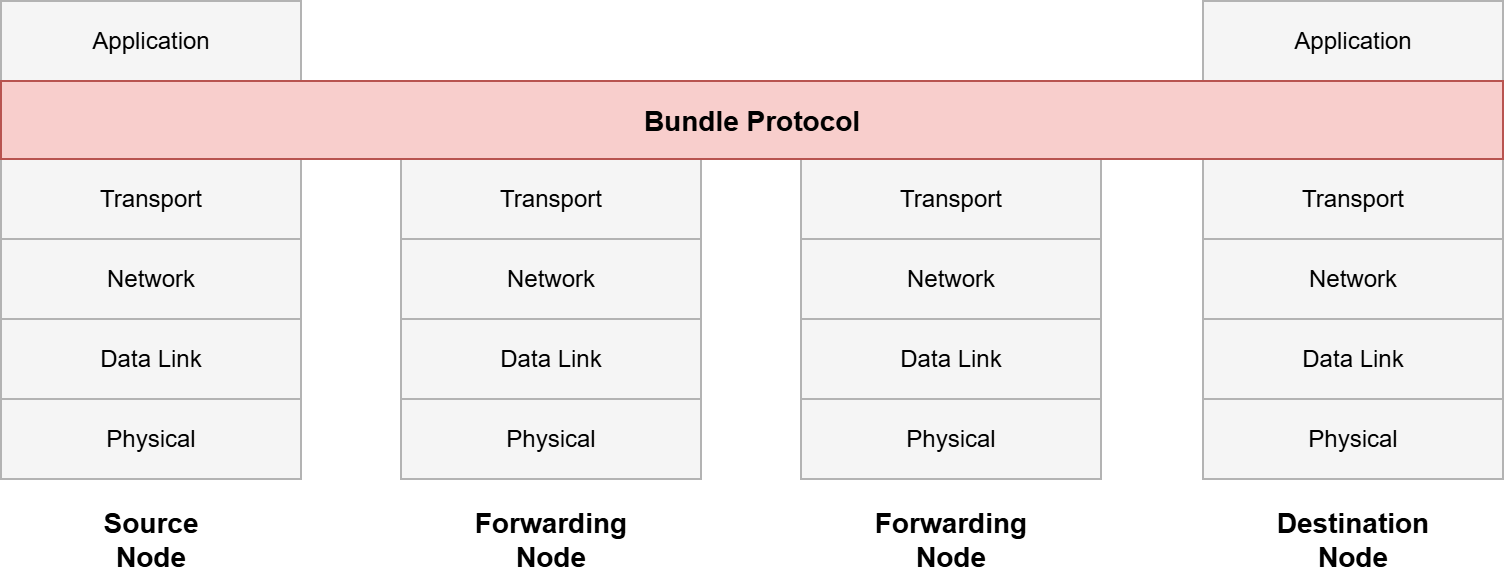
\includegraphics[width=\linewidth]{Literature Review/Typicall_DTN_implementation.png}
    \caption{Typicall DTN implementation}
    \label{Typicall_DTN_implementation}
\end{figure}

\section{Email System Architecture}

The traditional email system is a classic example of a distributed, store-and-forward system. It relies on a set of logical components and standardized protocols working in concert to enable global message delivery.

\subsection{Core Components}

\begin{figure}[h]
    \centering
    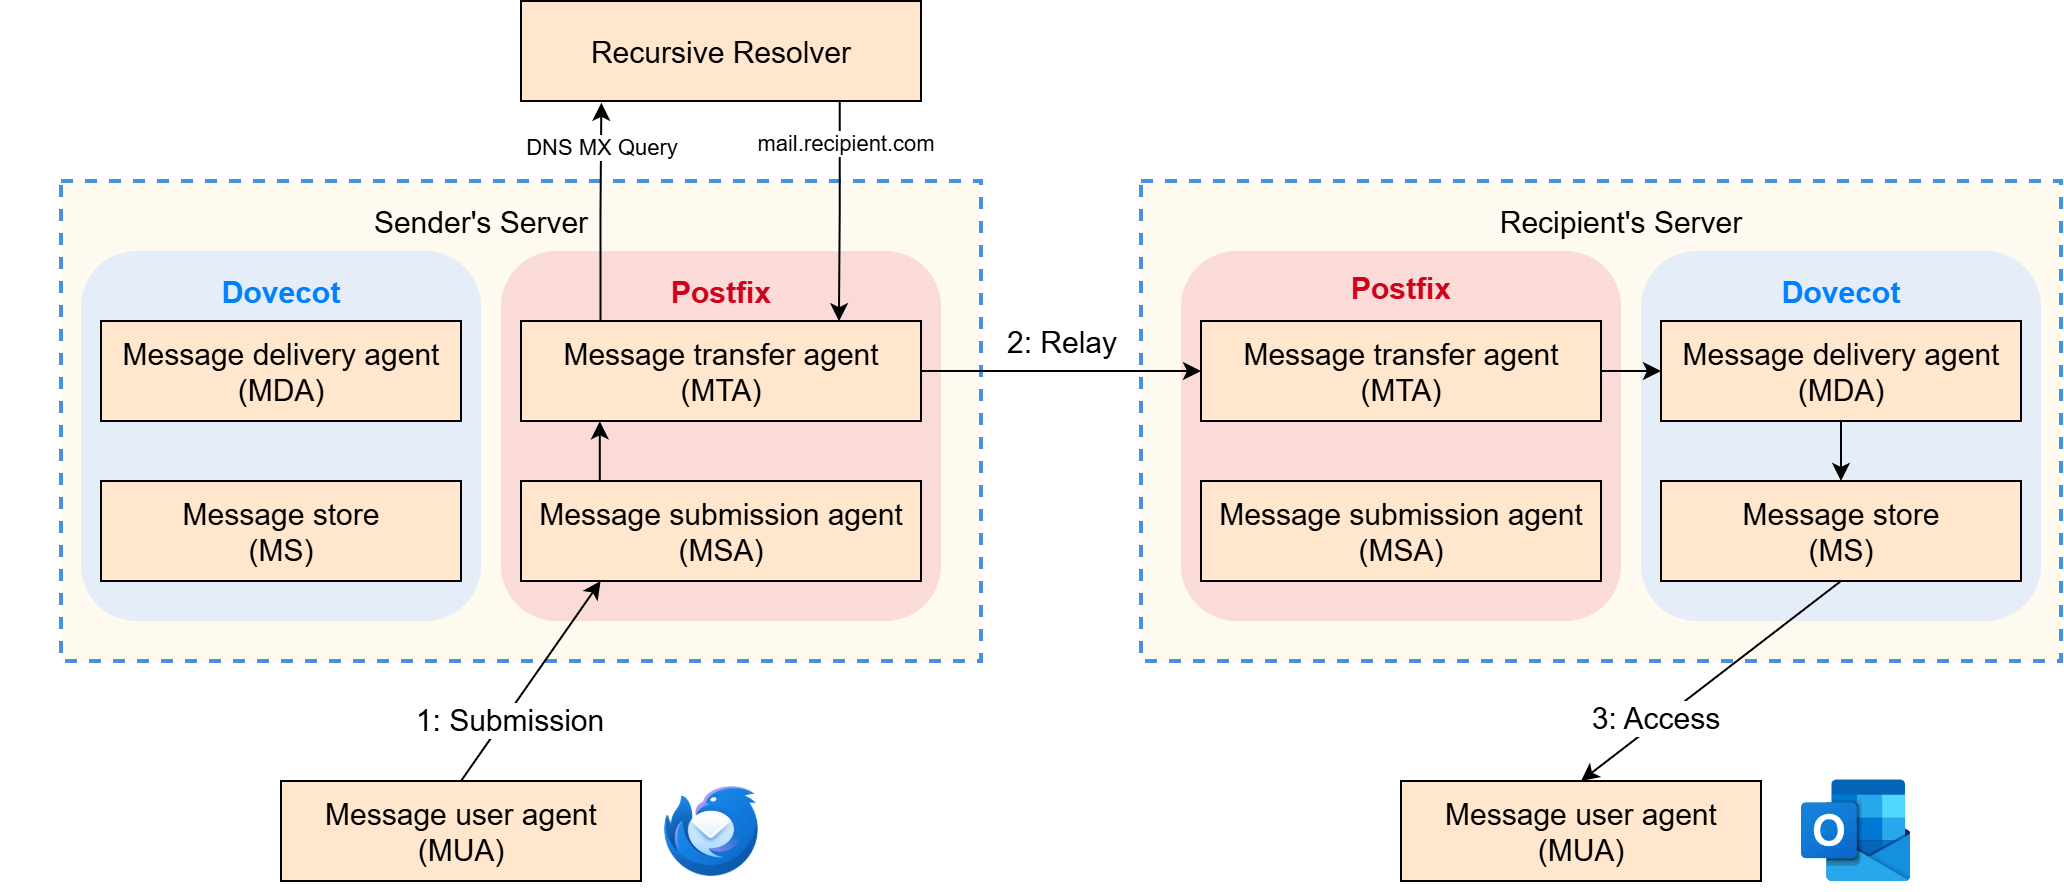
\includegraphics[width=\linewidth]{Literature Review/Email_architecture.png}
    \caption{Email architecture}
    \label{Email_architecture}
\end{figure}
As shown in Figure \ref{Email_architecture}, a typical email transaction involves the following core components~\cite{rfc5598}:

\begin{enumerate}
    \item Mail User Agent (MUA): This is the client software with which the user directly interacts, such as Mozilla Thunderbird or Microsoft Outlook. The MUA is responsible for composing, displaying, and managing emails, and it communicates with mail servers using standard protocols.
    \item Mail Submission Agent (MSA): The MUA submits an outgoing email to an MSA. The MSA authenticates the user, performs a preliminary check of the message format, and then passes the email to a Mail Transfer Agent (MTA). Typically, MSA functionality is provided by MTA software (e.g., Postfix) on a dedicated port (port 587).
    \item Mail Transfer Agent (MTA): The MTA is the central hub of the email system, acting as a ``post office.'' Examples include Postfix and Sendmail. Its primary responsibility is to relay emails from one server to another. It does this by looking up the Mail Exchange (MX) record in the DNS for the recipient's domain to find the next-hop MTA and then uses SMTP to forward the message.
    \item Mail Delivery Agent (MDA): When an email arrives at its final destination MTA, an MDA takes over. The MDA is responsible for placing the email into the appropriate user's mailbox. Software like Dovecot provides robust MDA functionality, including the ability to filter and sort incoming messages.
    \item Message Store: This is the physical or logical location on the server where emails are stored, representing the final, static destination in an email's lifecycle. It is a passive component, written to by the MDA and read from by the IMAP/POP3 server in response to MUA requests. The two most common storage formats are~\cite{MaildirSpec}:
    \begin{enumerate}
        \item mbox: Stores all of a user's emails concatenated into a single file. While simple to implement, this format suffers from performance issues with concurrent access and can pose challenges for data recovery.
        \item Maildir: Creates a separate file for each email, organized within a specific directory structure (e.g., cur, new, tmp). This format avoids file-locking issues, is more robust, and is the preferred choice in modern mail systems.
    \end{enumerate}
\end{enumerate}

\subsection{Key Protocols}

Communication between the components described above relies on the following key protocols:

\begin{enumerate}
  \item SMTP (Simple Mail Transfer Protocol)

  SMTP~\cite{rfc5321} is the standard protocol for sending and relaying email. It is a TCP-based, text-driven ``push'' protocol characterized by its highly conversational or interactive nature. A successful mail transfer involves a sequence of strictly ordered command-and-response interactions between client and server, such as: \texttt{EHLO/HELO} (greeting and identification), \texttt{AUTH} (authentication), \texttt{MAIL FROM} (sender's address), \texttt{RCPT TO} (recipient address), \texttt{DATA} (start of message content), and \texttt{QUIT} (termination). After each command, the client must wait for a three-digit status code (e.g., 250 OK) from the server before proceeding. This tightly coupled model requires low latency and stable network connections.
  \item POP3 (Post Office Protocol 3) / IMAP (Internet Message Access Protocol)

  These protocols are used by an MUA to retrieve and manage emails from a server. POP3~\cite{rfc1939} is a simple ``pull'' protocol that usually downloads all messages to the local client and deletes them from the server. IMAP~\cite{rfc9051} is more flexible, allowing server-side folder management and message status synchronization across multiple clients, with messages typically remaining stored on the server.

  \item TCP (Transmission Control Protocol)

  All of the above application protocols run over TCP, which strongly influence email system behavior and performance. TCP establishes a connection via a three-way handshake and guarantees in-order, lossless delivery using acknowledgments, retransmissions, and congestion control. These mechanisms introduce additional round trips beyond the application’s own command/response exchanges, making end-to-end latency directly visible to SMTP, POP3, and IMAP. Specifically: (a) connection setup/teardown incur RTT-dependent delays; (b) per-command turn-taking in SMTP/POP3/IMAP is serialized atop TCP’s flow, so each application step often waits at least one RTT; (c) TCP’s slow start and congestion control limit initial throughput and reduce the congestion window on loss, which can stall or stretch message transfers; (d) head-of-line blocking within a single TCP stream means that any lost segment pauses delivery of subsequent bytes, amplifying the impact of even modest packet loss when RTT is large. As a result, email protocols—especially SMTP’s highly interactive exchange and IMAP’s metadata-rich operations—perform best on low-latency, low-loss paths, while high RTT or intermittent loss can significantly degrade responsiveness, prolong sessions, and increase timeout/retry behavior.

  \item Anti-Spam and Authentication Mechanisms (via DNS Queries)

  To combat spam and phishing, a suite of protocols works alongside SMTP to verify sender identity. These protocols do not transfer message data themselves but leverage the DNS to publish and check authentication policies. 
  \begin{itemize}
    \item DNSBL (Domain Name System blocklist) check occurs the moment a sender's MTA connects, even before significant SMTP commands are exchanged. The recipient's MTA queries a DNS-based, real-time database of IP addresses known for sending spam. If the connecting IP is listed, the MTA can reject the connection outright.
    \item SPF (Sender Policy Framework) allows a domain to specify which MTAs are authorized to send email on its behalf. The recipient's MTA checks the IP address of the sender's MTA against this authorized list published in the domain’s DNS records. 
    \item DKIM (DomainKeys Identified Mail) provides message integrity by adding a digital signature to the email. The sender's MTA signs the message with a private key, and the recipient's MTA uses a corresponding public key from the DNS to verify that the message is authentic and has not been altered in transit. 
    \item DMARC (Domain-based Message Authentication, Reporting, and Conformance) unifies SPF and DKIM. It allows the sender's domain to set a policy that instructs the recipient's MTA on how to handle messages that fail these checks (e.g., to quarantine or reject them) and provides a reporting mechanism for monitoring.
  \end{itemize}
\end{enumerate}

In summary, the traditional email system is a complex ecosystem of components and interactive protocols. Its operation depends on the assumption of a low-latency and continuously available underlying network—namely, the TCP/IP-based Internet. This assumption makes it unsuitable for DTN.

\section{Solutions for DTN Email}
To adapt traditional email systems for DTN environments, a series of collaborative IETF drafts has been proposed. Together, they define a comprehensive solution by addressing three key aspects: service interaction, data format, and dependency resolution.

\subsection{Service Interaction}

Johnson Draft \cite{draft-johnson-dtn-interplanetary-smtp} proposes a solution centered on an SMTP gateway. Its core concept is to place a gateway between the DTN and a traditional TCP/IP network. This gateway acts as a protocol translator, converting TCP-based SMTP sessions into BP transmissions for outgoing mail, and reversing the process for incoming mail. This approach enables seamless integration between legacy mail servers and a DTN. The detailed workflow is as follows:

\begin{enumerate}
    \item \textit{Terminate SMTP Session}
    
    The gateway presents itself as a standard SMTP server to the local mail server (e.g., Postfix). When the local server attempts to send an email to a destination within the DTN, it establishes a standard SMTP connection with the gateway.
    \item \textit{Package Mail Transaction}
    
    The gateway engages in and completes the entire SMTP conversation, collecting all necessary information, including the sender, recipient(s), and the full message header and body.
    \item \textit{Trigger Bundle Encapsulation}
    
    The gateway then takes the complete mail transaction and triggers its encapsulation into one or more BP bundles, which are then dispatched into the DTN.
\end{enumerate}

This scheme provides excellent backward compatibility with existing email infrastructure. It effectively answers the question of how to interface with the DTN, but it does not specify the precise internal format of the encapsulated bundle.

\subsection{Data Format}

To complement and complete the gateway solution, the Blanchet Draft \cite{draft-blanchet-dtn-email-over-bp} was introduced. Rather than being a competing proposal, this draft provides a detailed technical specification for how an email should be encapsulated within a bundle, defining a standard format. Its key contributions include:

\begin{itemize}
    \item \textit{Data Model}
    
    Specifies how a standard email message (compliant with RFC 5322) should be mapped into a BP bundle.
    \item \textit{Block Definition}
    
    Recommends that the entire email, including headers and body, be placed either in the bundle's primary payload block or in a separate payload block.
    \item \textit{Metadata Mapping}
    
    Explores the possibility of mapping key email header fields (such as the Message-ID) to bundle metadata to facilitate more efficient processing.
\end{itemize}

Thus, these two drafts are complementary: the Johnson draft defines \textit{what} the gateway does (interacts with the SMTP world), while the Blanchet draft defines \textit{how} the gateway does it (generates a standardized email bundle). A complete, standards-compliant gateway implementation should adhere to both.

\subsection{Dependencies Resolution}

Email routing is critically dependent on DNS for resolving MX records. Standard DNS, however, is unworkable in a DTN environment. The Johnson DNS Draft \cite{draft-johnson-dtn-interplanetary-dns} addresses this crucial dependency by proposing a DTN-DNS gateway. This gateway intercepts local DNS queries, packages them into bundles for transmission across the DTN to an authoritative server, and returns the response, also in a bundle. This mechanism is fundamental to ensuring that the DTN email system can correctly route messages.

\section{The BPMail Gateway}

The value of theoretical drafts lies in their practical feasibility. The ASCENT project \cite{bpmail}, initiated by California State University, developed an open-source tool called BPMail, which is a concrete implementation of the gateway concept. BPMail is designed to integrate with the Postfix mail system as a custom mail delivery agent.

BPMail's workflow aligns closely with the behavior described in the Johnson draft. It is invoked by Postfix, receives a complete email message, and then uses the library functions of ION-DTN (a leading DTN protocol stack developed by NASA) to encapsulate the email into a bundle and inject it into the local ION node. BPMail provides practical validation for the theoretical proposals, and its encapsulation process represents the core operation that the Blanchet Draft aims to standardize. Therefore, BPMail serves as an ideal tool for researching and simulating a complete DTN email system based on this series of drafts.

\section{Summary}

In summary, the existing literature has established a clear and collaborative technical framework for enabling email communication in DTN environments. The technology roadmap, from the analysis of space network requirements to the development of the DTN architecture and a series of complementary standardization drafts, is well-defined. The existence of practical tools like BPMail further demonstrates the framework's feasibility.

However, a significant gap remains in the current body of research: most literature focuses on architectural design and qualitative feasibility, lacking a systematic analysis of the scheme's limitations within a simulated software environment.

Specifically, the following questions have not been adequately addressed:

\begin{itemize}
    \item \textit{Architectural Limitation (User Mobility)}
    
    Current gateway solutions implicitly assume that a user's access point (i.e., their DTN gateway node) is static. The schemes do not consider how email routing and addressing should be dynamically managed when a user travels between celestial bodies or large habitats.
    \item \textit{Implementation Limitation (Handling of Large Attachments)}
    
    A theoretical scheme must be realized through software, which may itself have bottlenecks. For example, the performance, resource consumption, and potential failure points of a core tool like BPMail when handling large attachments need to be evaluated to determine the scheme's practical utility.
\end{itemize}

Therefore, the value of this dissertation lies in filling this gap. By simulating and replicating a complete DTN email system in a highly controlled, containerized environment, this research aims to conduct an analysis of its potential limitations, thereby providing valuable data and insights for its future optimization and deployment.

\chapter{Experimental Methods}
\section{Materials}

\section{Synthetic Procedures}
\subsection{Parameters Varied}

\section{Characterisation Techniques}
\subsection{A}
\subsection{B}
\subsection{C}
\subsection{D}
\chapter{Results and Discussion}
This chapter presents and analyzes the results from experiments conducted on the simulation platform described previously.  
The chapter begins by reviewing the system's normal workflow in a standard scenario, which serves as a baseline for analysis.  
Subsequently, it introduces a more challenging ``user interplanetary mobility'' scenario.  
Through quantitative test data, this section reveals the performance limitations inherent in the current Johnson Draft when applied to this scenario.
Finally, based on an discussion of these limitations, the chapter offers a conceptual proposal to address the challenges.

\section{Baseline Scenario Review}

In its standard scenario, email transmission and reception rely entirely on the DTN gateway for relay.  
For instance, when a user on Earth sends an email to a user on the Moon, the message is submitted to the local \texttt{mail-1}.  
There, the \texttt{BPMailSend} gateway component encapsulates it into a bundle, which is then transmitted asynchronously and reliably over the DTN link to \texttt{mail-2}.  
Upon arrival, the \texttt{BPMailRecv} component decapsulates the bundle and delivers the email to the end user.  
In this scenario, interactive experience is seamless, as the high-latency interplanetary link is effectively shielded by the DTN gateway and the Bundle Protocol.

\section{User Interplanetary Mobility Scenario}

\subsection{Scenario Description and Problem Analysis}

A core assumption of existing DTN email gateway proposal is that the user's MUA and their home MTA/MDA are located within the same low-latency ``local'' network.  
However, this raises a practical and important question: how should users access their email when they travel between celestial bodies?

The key test scenario designed in this dissertation is as follows: a user whose home mailbox is on the Moon (located on \texttt{mail-2}) travels to Earth for a mission.  
From Earth, the user attempts to connect to and synchronize all the emails from their home server on the Moon using a local device (\texttt{client-1}).

In this scenario, a problem immediately becomes apparent.  
As depicted in Figure~\ref{fig:mobility_scenario}, the user's Thunderbird client is configured to connect directly to their home server \texttt{mail-2}.
Because \texttt{mail-2} is located on the distant Moon, this IMAP connection request must traverse the entire long-latency interplanetary link.  
The DTN gateway is completely bypassed in this process because IMAP is an end-to-end, TCP-based, real-time synchronization protocol that cannot be handled by an gateway like BPMail.


\begin{figure}[ht]
      \centering
      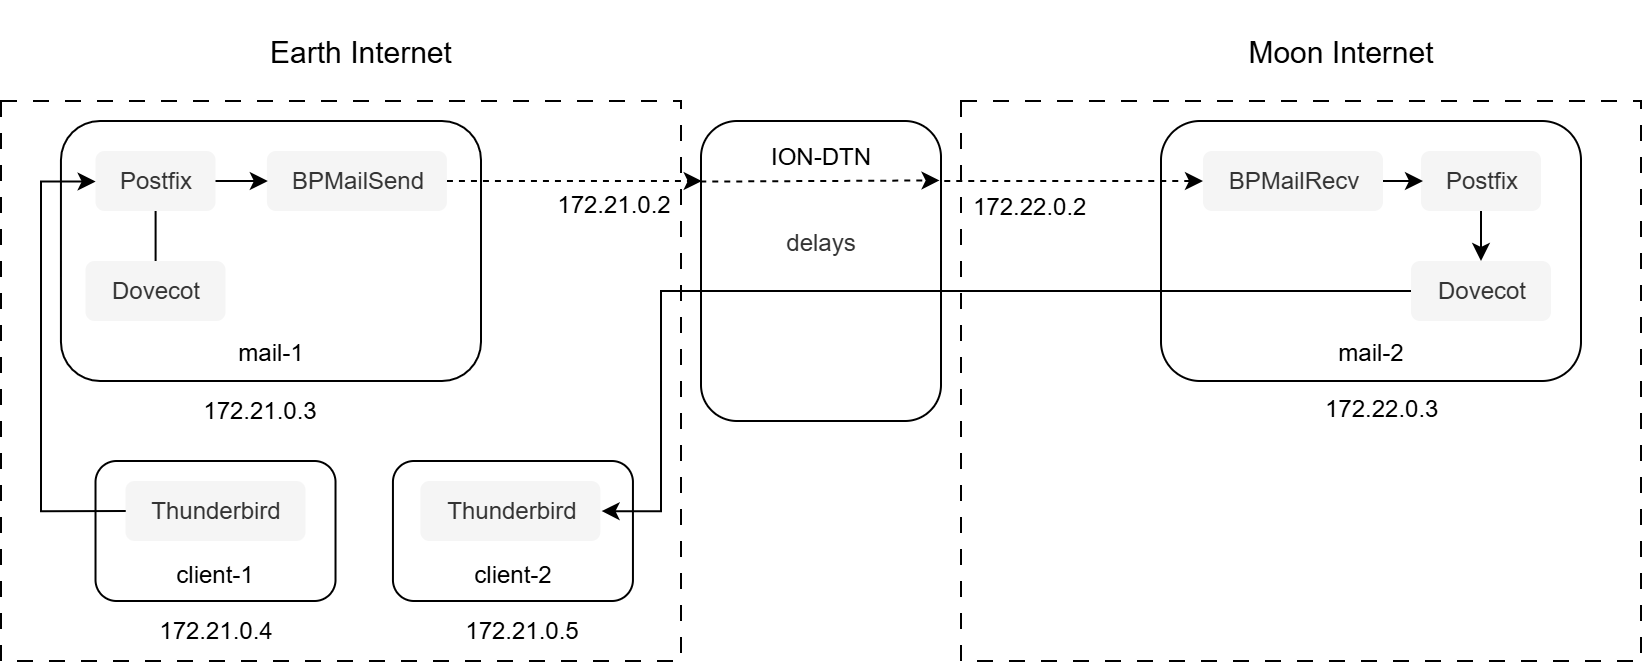
\includegraphics[width=1.0\textwidth]{Results/mobility_scenario.png}
      \caption{Illustration of the mobility scenario}
      \label{fig:mobility_scenario}
\end{figure}

\subsection{Experimental Results}
To quantify the impact of this problem, an experiment was conducted to measure the total time required for a client on Earth to synchronize 1000 simple emails (with the body ``Hello'') from the server on the Moon under various network delays.  
The results are presented in Table~\ref{tab:email-retrieval-time}.

\begin{table}[ht]
\centering
\setlength{\tabcolsep}{10pt}
\caption{Email retrieval time under different delays}
\label{tab:email-retrieval-time}
\begin{tabular}{cccc}
\hline
\textbf{Delay (s)} & \textbf{Body} & \textbf{Number of Emails} & \textbf{Retrieval Time (s)} \\
\hline
0   & "Hello" & 1000 & 19  \\
1   & "Hello" & 1000 & 33  \\
2   & "Hello" & 1000 & 64  \\
5   & "Hello" & 1000 & 153 \\
0   & "Hello" with attachment & 1 & Time out \\
\hline
\end{tabular}
\end{table}

As is clearly evident from Table~\ref{tab:email-retrieval-time}, the email retrieval time deteriorates sharply as the one-way delay increases.  
In a zero-delay environment (equivalent to a local area network), retrieving the emails takes only 19 seconds.  
However, when the delay reaches 5 seconds, completing the synchronization requires 153 seconds (over two and a half minutes).  
At this point, the user experience becomes unacceptable, and the system is rendered effectively unusable.

\section{Discussion and Limitation Analysis}

The experimental results above reveal multiple limitations in the design of the Johnson Draft.

\subsection{Architectural Limitation}

The data provides direct evidence of the proposal's failure to support user interplanetary mobility.  
The effectiveness of this solution is predicated on decoupling real-time user interaction (Client--Server) from asynchronous server-to-server relay (Server--Server) and applying DTN technology only to the latter.  
When a user roams, the client--server interaction, which is supposed to occur over a local, low-latency network, is forced to traverse a long-latency interplanetary link.  
This negates the delay-tolerant advantages of the entire system.  
The performance collapse is caused by ``chatty'' protocols like IMAP and SMTP, which require numerous round-trips that are severely penalized by high latency.

\subsection{Implementation Limitation}

During testing, a significant bottleneck was identified in the practical application of the current proposal: the BPMail gateway implementation is incapable of correctly processing emails with large attachments.

When attempting to send an email with a moderately large attachment (e.g., 3\,MB) through the gateway, the mail delivery fails.  
The likely cause of this issue lies within the memory management mechanisms of the BPMail software itself.  
For instance, the program may attempt to read the entire email content into a fixed-size memory buffer.  
When the email size exceeds this buffer's capacity, a buffer overflow or memory allocation failure occurs.

This implementation flaw severely limits the practical utility of the solution.  
In modern communication, email serves not only as a medium for text but also as a crucial tool for exchanging files and data.  
An email system that cannot handle a 3\,MB attachment is unacceptable for many real-world applications.



\section{Discussion of Extension}

To address the limitations identified above, particularly the challenges related to user mobility, this section proposes a conceptual extension informed by existing research in related fields.

In fact, the problem identified in this research falls under the broader category of ``Mobility Management'' within the field of DTN.  
Existing research has generally pursued solutions at two distinct layers:

\begin{itemize}
    \item \textbf{The Network Layer}: This approach aims to provide transparent mobility support through mechanisms such as dynamic routing protocols or directory services that track the changing locations of mobile nodes and route data accordingly.
    \item \textbf{The Application Layer}: This approach focuses on using proxies or caches to confine real-time user--service interactions to the local network, while handling data synchronization asynchronously in the background. Concepts like ``Data Mules'' are a classic example of this application-layer data ferrying philosophy.
\end{itemize}

Given the immense complexity of network-layer solutions, an application-layer proxy approach represents a more pragmatic and readily achievable path.
To this end, this dissertation proposes the \textit{On-demand Sync Agent} extension, a specific conceptualization of an application-layer solution.  
Its architecture is depicted in Figure~\ref{fig:sync_agent}.

\begin{figure}[ht]
      \centering
      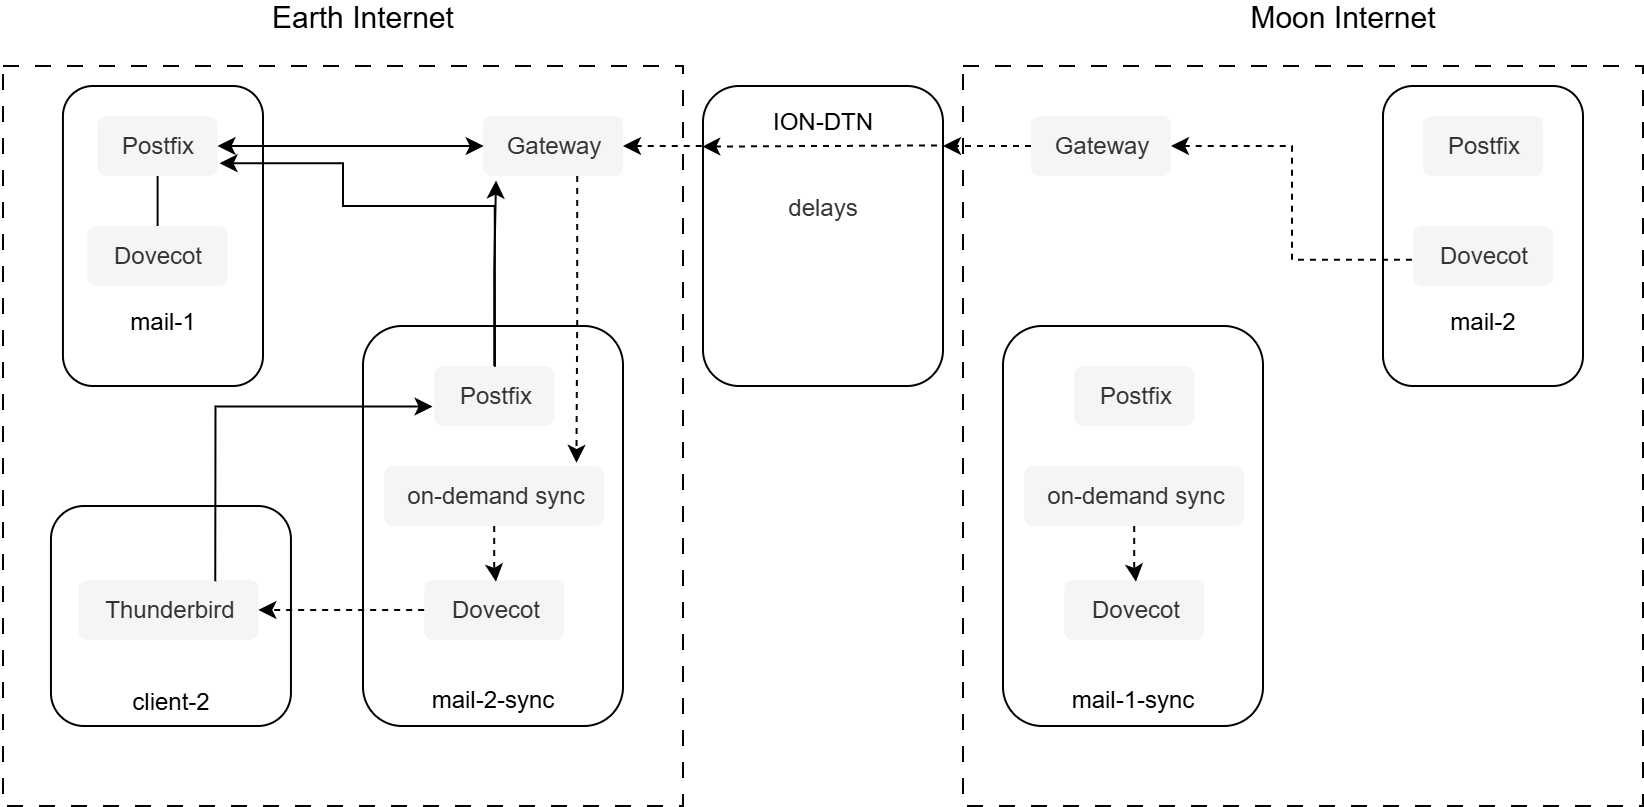
\includegraphics[width=1.0\textwidth]{Results/sync_agent.png}
      \caption{Conceptual Extension of the On-demand Sync Agent}
      \label{fig:sync_agent}
\end{figure}

The operational logic of this conceptual architecture is as follows:

\begin{enumerate}
    \item \textit{Introduction of a Local Sync Agent}: A ``Sync Agent'' service is deployed on each celestial body (e.g., Earth). To the user, this service appears as a fully functional, local mail server.
    \item \textit{Localization of User Interaction}: A roaming user (e.g., a user from the Moon who has traveled to Earth) configures their Thunderbird client to connect to this local Sync Agent on Earth, not to their distant home server on the Moon. This ensures a seamless and responsive user experience.
    \item \textit{Background DTN Synchronization}: The Sync Agent is responsible for conducting batch, asynchronous email synchronization with the user's home server (e.g., \texttt{mail-2} on the Moon) in the background. All data that must cross the interplanetary link is handled by the agent, which encapsulates it into bundles for transmission via the DTN gateway.
\end{enumerate}

This conceptual extension decouples the user's real-time interactions from the background data synchronization by introducing an intermediary proxy layer.
It thus holds potential to resolve the performance issues caused by user roaming.

It must be emphasized, however, that this is a preliminary architectural concept intended to inspire future research.  
It still faces significant challenges — for example, the proposed "Sync Agent" would require email service providers to pre-deploy servers on other planets, which poses considerable implementation difficulties.

\section{Summary}

By designing and testing a key ``user interplanetary mobility'' scenario, this chapter has identified and validated limitations of the existing DTN email gateway proposal.  

First, experimental data demonstrated that direct access to a remote mail server in a roaming scenario leads to severe performance degradation.  
Second, functional testing revealed that the core BPMail gateway component is unable to handle large attachments.  

Following a discussion of these limitations, this chapter proposed an extension based on an \textit{Sync Agent}, and revealed its shortcomings as well.

\chapter{Conclusions and Future Work}
\section{Conclusion}

This dissertation has completed a simulation and analysis of a modern delay-tolerant email proposal.  
In the implementation phase, a simulation platform was established based on Docker containerization, integrating a mail server (Postfix/Dovecot), a client (Thunderbird), a DTN protocol stack (ION-DTN), an email gateway (BPMail), and a network simulator (\texttt{tc}).

During the experimental testing phase, a key ``user interplanetary mobility'' roaming scenario was designed and validated.  
The test results revealed a architectural flaw in the proposal: when a user roams to a remote network and attempts to access their home mail server, the real-time synchronization protocols (IMAP/SMTP) are forced to operate over a long-latency link.
This leads to a sharp performance degradation that renders the system unusable, demonstrating that the Johnson Draft does not support user mobility.  

Furthermore, functional testing identified an implementation deficiency in the BPMail gateway component, which was unable to process large attachments, thereby limiting its practical value.

To address the mobility issue, this research proposed a conceptual extension based on an \textit{Sync Agent}.  
This extension decouples the user's real-time interaction with the email system from background data synchronization across interplanetary links by establishing a local agent, offering a potential solution to this limitation.

\section{Limitations}

Although this research achieved its primary objectives, it is subject to the following limitations:

\begin{itemize}
    \item \textit{Simplified Network Environment Simulation}: The simulation primarily focused on long delay, the most prominent characteristic of deep-space networks. Other complex network conditions, such as bit error rates, asymmetric bandwidth, and periodic disruptions, were not extensively tested in combination.
    \item \textit{Lack of DNS and Security Mechanism Simulation}: To focus on the core issues of mail transport and synchronization, the implementation simplified the DNS server configuration. Consequently, it was not possible to experimentally validate the potential failure of DNS-dependent email trust mechanisms (e.g., SPF, DKIM) in the roaming scenario.
    \item \textit{Unverified Nature of the Proposed Extension}: The \textit{On-demand Sync Agent} extension presented in this dissertation remains at the conceptual design stage. Its effectiveness, and any new issues it might introduce (such as implementation difficulties) have not been verified through prototype implementation.
\end{itemize}

\section{Future Work}

Based on the findings and limitations of this research, several avenues for future work can be identified:

\begin{itemize}
    \item \textit{Improving DTN Gateway Support for Large Files}: The most direct and practically valuable line of future work would be to address the shortcomings of BPMail. This could involve debugging and patching its source code or developing a new, more robust mail gateway to ensure reliable handling of large attachments, thereby removing a key barrier to the proposal's practical deployment.
    \item \textit{Implementation and Validation of the Proposed Solution}: The next logical step is to transform the \textit{On-demand Sync Agent} extension from a concept into a reality. This would involve developing a prototype system and deploying it on the simulation platform to evaluate its performance in user roaming scenarios.
    \item \textit{Testing Under More Adverse Network Conditions}: The existing simulation platform could be extended to more complex network environment. By simulating a combination of delay, jitter, packet loss, and disruptions, a more comprehensive stress test could be conducted to evaluate the ultimate performance and robustness of DTN email proposals.
\end{itemize}

\chapter{Figures, Tables, Referencing}
It is very important to properly refer in the text to any figures, tables or previously published work that you are discussing. Adequate and consistent referencing is one of the criteria which will be used to assess your project report.

\section{Figures}
Graphs, pictures and other images should be included in your report as a numbered, captioned figure. An example is given in Figure \ref{veldis}.

%%%%%%%%%%%%%%%%%%%%%%%%%%%%%%%%%%%%%%%%
\begin{figure}[h]
      \centering
      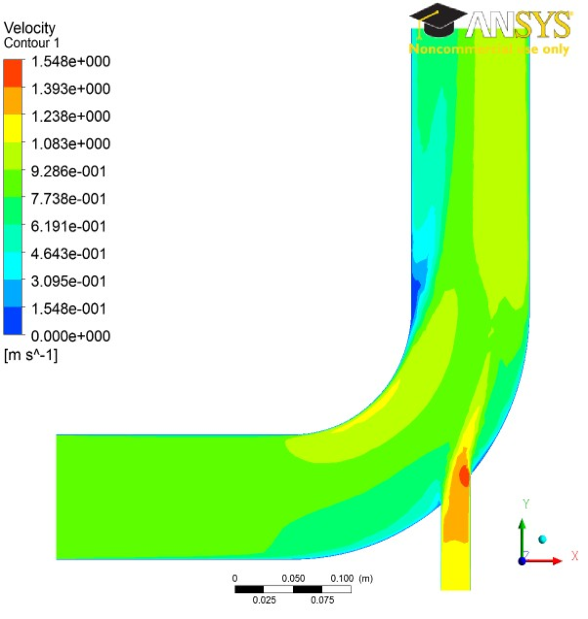
\includegraphics{background/5e1-1.pdf}
      \caption{Velocity distribution on the mid-plane for an inlet velocity for case 1.}
      \label{veldis}
\end{figure}
%%%%%%%%%%%%%%%%%%%%%%%%%%%%%%%%%%%%%%%%

The figure and caption should be centred. The figure numbering starts at 1 at the beginning of each chapter. The caption should provide a brief description of what is being shown. The figure should appear in the document after it is referred to in the text. No figure should be included which is not referred to in the text. Ensure that the size and resolution of images imported from software are sufficient to read any text.

\section{Tables}
Tables are an important way of displaying your results. Table \ref{tab:treatments} is a sample table, adapted from the Master/Doctoral Thesis template at \url{http://www.latextemplates.com/cat/theses}, which was generated with this code:

{\footnotesize
\begin{verbatim}
\begin{table}[b]
\caption{The effects of treatments X and Y on the four groups studied.}
\label{tab:treatments}
\centering
\begin{tabular}{l l l}
\toprule
\textbf{Groups} & \textbf{Treatment X} & \textbf{Treatment Y} \\\midrule
1 & 0.2 & 0.8\\
2 & 0.17 & 0.7\\
3 & 0.24 & 0.75\\
4 & 0.68 & 0.3\\
\bottomrule\\
\end{tabular}
\end{table}
\end{verbatim}
}

\begin{table}[b]
\caption{The effects of treatments X and Y on the four groups studied.}
\label{tab:treatments}
\centering
\begin{tabular}{l l l}
\toprule
\textbf{Groups} & \textbf{Treatment X} & \textbf{Treatment Y} \\
\midrule
1 & 0.2 & 0.8\\
2 & 0.17 & 0.7\\
3 & 0.24 & 0.75\\
4 & 0.68 & 0.3\\
\bottomrule\\
\end{tabular}
\end{table}

Tables are numbered in the same way as figures. Typically tables also have a short caption, but this is not universally true. The number and caption appear above the table, not below as with figures. Again, no table should appear in the report which has not been referred to in the text. Tables should come after they are discussed in the text. The exact formatting of the table depends somewhat on the content of the table, but in general, the text in the table should be the same font and size as the main text. 

\section{Equations}
All equations should be numbered sequentially. Do not restart the numbering at the beginning of each chapter. Unlike figures and tables, you may not need to refer to every equation in the text. You should take care to format equations properly. Do no simply try to use plain text. Use the equation layout facilities. An example of how equations should appear is shown in Equation \ref{sampleequation}. Here is the code for it:

{\footnotesize
\begin{verbatim}
\begin{equation}
\textrm{div}(\underline{u}) = \frac{\delta u}{\delta x} + \frac{\delta v}{\delta y} +
        \frac{\delta w}{\delta z} = 0
\label{sampleequation}
\end{equation} 
\end{verbatim}
}

\begin{equation}
\textrm{div}(\underline{u}) = \frac{\delta u}{\delta x} + \frac{\delta v}{\delta y} + \frac{\delta w}{\delta z} = 0
\label{sampleequation}
\end{equation} 

\section{Referencing published work}
It is important to give appropriate credit to other people for the work that they have shared through publications. In fact, you must sign a declaration in your report stating that you understand the nature of plagiarism. As well as avoiding plagiarism, citing results or data from the literature can strengthen your argument, provide a favourable comparison for your results, or even demonstrate how superior your work is.

There are many styles to reference published work. For example, the parenthetical style (which is also called the \emph{Harvard style}) uses the author and date of publication (e.g. ``Smith and Jones, 2001''). There is also the Vancouver style (or the \emph{citation sequence style}), which is used in this document. In the Vancouver style, the publications are cited using bracketed numbers which refer to the list in the References section at the end of the report. The references are listed in the order that they are cited in the report. A variant is \emph{name sequence style}, in which the publications are referenced by number, but the list is arranged alphabetically. The following paragraph shows the use of the Vancouver style: 

\begin{quote}
Several studies have examined the sound field around tandem cylinders generated by flow\cite{fitzpatrick2003flow,finnegan2010experimental}, while other investigations have focused on the effect of an applied sound field on the flow\cite{hall2003vortex}. Papers from conference proceedings\cite{jordan2001array}, books\cite{paidoussis2010fluid} and technical reports\cite{reyes2007power} can be dealt with in the same style.
\end{quote}

The Vancouver style has the advantage that it is a little more compact in the text and does not distract from the flow of the sentence if there are a lot of citations. However, it has the disadvantage that it is not immediately clear to the reader what particular work has been referenced.

It actually does not matter which particular referencing style is used as long as three important considerations are observed:
\begin{itemize}
\item the referencing style used throughout the document is consistent;
\item all material used or discussed in the text is properly cited;
\item nothing is included in the reference list that has not been cited.
\end{itemize}

This template has a suitable referencing style already set up -- you should use it and use the built-in BibTeX system to manage your references. See above for examples of how to cite a reference and look in the \texttt{sample.bib} file to see BibTeX references. Remember \href{http://scholar.google.com}{Google Scholar} and other search engines will give you BibTeX references for lots of academic publications. Otherwise, you can easily make up your own based on the examples in that file.
\chapter{\LaTeX}
\label{latexchapter}
\LaTeX{}, or more properly ``\LaTeXe{}'', is a very useful document processing program. It is very widely used, widely available, stable and free. Famously, \TeX, upon which \LaTeX{} is built, was originally developed by the eminent American mathematician Donald Knuth because he was tired of ugly mathematics books \cite{shustek2008interview}. Although it has a learning curve (made much less forbidding by online tools and resources -- see below), it allows the writer to concentrate more fully on the content, and takes care of most everything else.

While it can be used as a word processor, it is a \emph{typesetting} system, and Knuth's idea was that it could be used to produce beautiful looking books:
\begin{quote}
\emph{\LaTeX{} is a macro package which enables authors to typeset and print their work at the highest typographical quality, using a predefined, professional layout.}\footnote{This is from \citet{oetiker2001not}. Did we mention that you should minimise your use of footnotes?}
\end{quote}
\LaTeX{} has great facilities for setting out equations and a powerful and very widely supported bibliographic system called BibTeX, which takes the pain out of referencing.

Three useful online resources make \LaTeX~much better:
\begin{enumerate}[(1)]
\item An excellent online \LaTeX{} environment called ``Overleaf'' is available at \url{http://www.overleaf.com} and runs in a modern web browser. It's got this template available -- search for a TCD template. Overleaf can work in conjunction with Dropbox, Google Drive and, in beta, GitHub.
\item Google Scholar, at \url{http://scholar.google.com}, provides BibTeX entries for most of the academic references it finds.
\item An indispensable and very fine introduction to using \LaTeX{} called \emph{``The not so short introduction to LATEX 2$\varepsilon$''} by \citet{oetiker2001not} is online at \url{https://doi.org/10.3929/ethz-a-004398225}. Browse it before you use \LaTeX~for the first time and  read it carefully when you get down to business.
\end{enumerate}
Other tools worth mentioning include:
\begin{itemize}
\item \texttt{Draw.io} -- an online drawing package that can output PDFs to Google Drive -- see \url{https://www.draw.io}.
\end{itemize}
\bibliographystyle{unsrtnat}
\bibliography{bibs/sample}
\appendix
\renewcommand{\thechapter}{A\arabic{chapter}}
\chapter{Appendix}
You may use appendices to include relevant background information, such as calibration certificates, derivations of key equations or presentation of a particular data reduction method. You should not use the appendices to dump large amounts of additional results or data which are not properly discussed. If these results are really relevant, then they should appear in the main body of the report.

\section{Appendix numbering}
Appendices are numbered sequentially, A1, A2, A3\ldots The sections, figures and tables within appendices are numbered in the same way as in the main text. For example, the first figure in Appendix A1 would be Figure A1.1. Equations continue the numbering from the main text.



\end{document}